% 质心 质心系
% 质心|质心系|参考系|重心

\pentry{体积分\upref{IntN}, 质点系\upref{PSys}}

\subsection{质心的定义}
质心通俗来讲可以理解为质量的中心, 是系统中各个质点的位置矢量\upref{Disp}关于质量的加权平均值. 我们先看几个例子.

\subsection{两个等质量质点的质心}
对于两个质量相等的质点, 它们的质心显然在它们连线的中点处, 无论它们的质量是多少. 如果它们都在 $x$ 轴上, 则质心的位置就是两质点 $x$ 坐标的中点
\begin{equation}\label{CM_eq2}
x_c = (x_1 + x_2)/2
\end{equation}
其中角标 c 表示 center of mass, 有时候也会写做 CM.

在二维和三维空间的情况下, 质点的位置用位置矢量 $\bvec r$ 描述, 将它们的位置矢量分别记为 $\bvec r_1$ 和 $\bvec r_2$, 则质心的位置为
\begin{equation}\label{CM_eq3}
\bvec r_c = (\bvec r_1 + \bvec r_2)/2
\end{equation}
即两个位置矢量的平均值. % 图未完成

\subsection{两个不同质量质点的质心}
当两个质点质量不一样时(分别记为 $m_1$ 和 $m_2$), 质心会更靠近更重的质点. 如果它们都在 $x$ 轴上, 我们就用加权平均值
\begin{equation}
x_c = \frac{m_1 x_1 + m_2 x_2}{m_1 + m_2}
\end{equation}
注意 $m_1 = m_2$ 就得到了\autoref{CM_eq2}. 另一个极端是当一个质量远大于另一个, 如 $m_1 \gg m_2$, 这时质心就趋近于 $x_1$ 了.

二维和三维空间的情况下也类似有
\begin{equation}\label{CM_eq5}
\bvec r_c = \frac{m_1 \bvec r_1 + m_2 \bvec r_2}{m_1 + m_2}
\end{equation}
当 $m_1 = m_2$ 就得到\autoref{CM_eq3}.

\begin{exercise}{}
证明两质点的质心必定在其连线上, 即 $\bvec r_1 - \bvec r_c$ 和 $\bvec r_2 - \bvec r_c$ 共线.% 共线如何证明? “几何矢量” 中有提吗?
\end{exercise}

\begin{exercise}{}
试证明\autoref{CM_eq5} 中质心到两质点的距离与它们的质量成反比, 即
\begin{equation}\label{CM_eq6}
\frac{\abs{\bvec r_1 - \bvec r_c}}{\abs{\bvec r_2 - \bvec r_c}} = \frac{m_2}{m_1}
\end{equation}
\end{exercise}

\subsection{质点系的质心}
若质点系中有 $N$ 个质点,令第 $i$ 个质点质量为 $m_i$,位置为 $\bvec r_i$,总质量为 $M = \sum\limits_i m_i$, 则该质点系的\textbf{质心}定义为
\begin{equation}\label{CM_eq1}
\bvec r_c = \frac{1}{M}\sum_i m_i \bvec r_i
\end{equation}

在直角坐标系中, 我们可以将上式的矢量求和分解为对 $x, y, z$ 方向的分量分别求和(因为矢量相加等于两个分量分别相加). 令 $\bvec r_i = x_i \uvec x + y_i \uvec y + z_i \uvec z$, 即矢量 $\bvec r_i$ 的坐标为 $(x_i, y_i, z_i)$, 有
\begin{equation}\label{CM_eq11}
x_c = \frac{1}{M}\sum_i m_i x_i \qquad
y_c = \frac{1}{M}\sum_i m_i y_i \qquad
z_c = \frac{1}{M}\sum_i m_i z_i
\end{equation}

\begin{example}{}
空间直角坐标系中四个质点质量分别为 $1 \Si{kg}$, $2 \Si{kg}$, $3 \Si{kg}$, $4 \Si{kg}$, 坐标分别为 $(0, 0, 0)$, $(1, 0, 0)$, $(0, 2, 0)$, $(0, 0, 3)$ (单位:米). 求该系统质心的位置.

解: 系统总质量为 $10 \Si{kg}$, 直接使用\autoref{CM_eq11} 得
\begin{equation}
x_c = \frac{1}{10 \Si{kg}} (0 \Si{m} \times 1 \Si{kg} + 1 \Si{m}\times 2 \Si{kg} + 0\Si{m} \times 3 \Si{kg} + 0 \Si{m}\times 4 \Si{kg}) = \frac15 \Si{m}
\end{equation}
\begin{equation}
y_c = \frac{1}{10 \Si{kg}} (0\Si{m}\times 1 \Si{kg} + 0\Si{m} \times 2 \Si{kg} + 2\Si{m} \times 3 \Si{kg} + 0 \Si{m}\times 4 \Si{kg}) = \frac35 \Si{m}
\end{equation}
\begin{equation}
z_c = \frac{1}{10 \Si{kg}} (0\Si{m}\times 1 \Si{kg} + 0\Si{m} \times 2 \Si{kg} + 0\Si{m} \times 3 \Si{kg} + 3 \Si{m}\times 4 \Si{kg}) = \frac65 \Si{m}
\end{equation}
所以质心的坐标为 $(1/5, 3/5, 6/5)$ (单位: 米).
\end{example}

\subsection{质心的分解}
若我们把质点系划分为若干组, 可以先计算每组的质心, 再计算 “质心的质心” 就可以得到系统的总质心. 我们举例说明
\begin{example}{}
令四个质点中的前两个为 $a$ 组, 后两个为 $b$ 组, 则它们的质心分别为
\begin{equation}
\bvec r_a = (m_1 \bvec r_1 + m_2 \bvec r_2)/M_a
\qquad
\bvec r_b = (m_3 \bvec r_3 + m_4 \bvec r_4)/M_b
\end{equation}
其中 $M_a = m_1 + m_2$, $M_b = m_3 + m_4$. 再计算 “质心的质心” 得整个系统的质心为
\begin{equation}
\bvec r_c = \frac{M_a \bvec r_a + M_b \bvec r_b}{M_a + M_b} = \frac{m_1 \bvec r_1 + m_2 \bvec r_2 + m_3 \bvec r_3 + m_4 \bvec r_4}{m_1 + m_2 + m_3 + m_4}
\end{equation}
这个结果符合\autoref{CM_eq1}.
\end{example}

\subsection{质心与重心}
质心在物理中有什么用呢? 一个基本的应用就是质心就是物体的\textbf{重心}. 我们只讨论恒定重力场中物体的重心. 其定义是: 若重力场对物体关于某点的合力矩\upref{Torque}恒为 0, 这个点就是它的\textbf{重心}. “合力矩为零” 意味着, 如果物体初始时以任意姿态静止, 那么它将一直保持静止. 虽然我们还没系统学习力矩, 但可以用初中学过的 “力乘力臂” 进行计算(\autoref{Torque_eq2}\upref{Torque}).

\begin{example}{}\label{CM_ex1}
轻杆\footnote{轻杆是指质量可忽略不计的杆}两端有质量分别为 $m_1$ 和 $m_2$ 的小球, 轻杆可以绕系统质心在竖直平面上自由转动. 试证明重力对系统的力矩恒为 0.

\begin{figure}[ht]
\centering
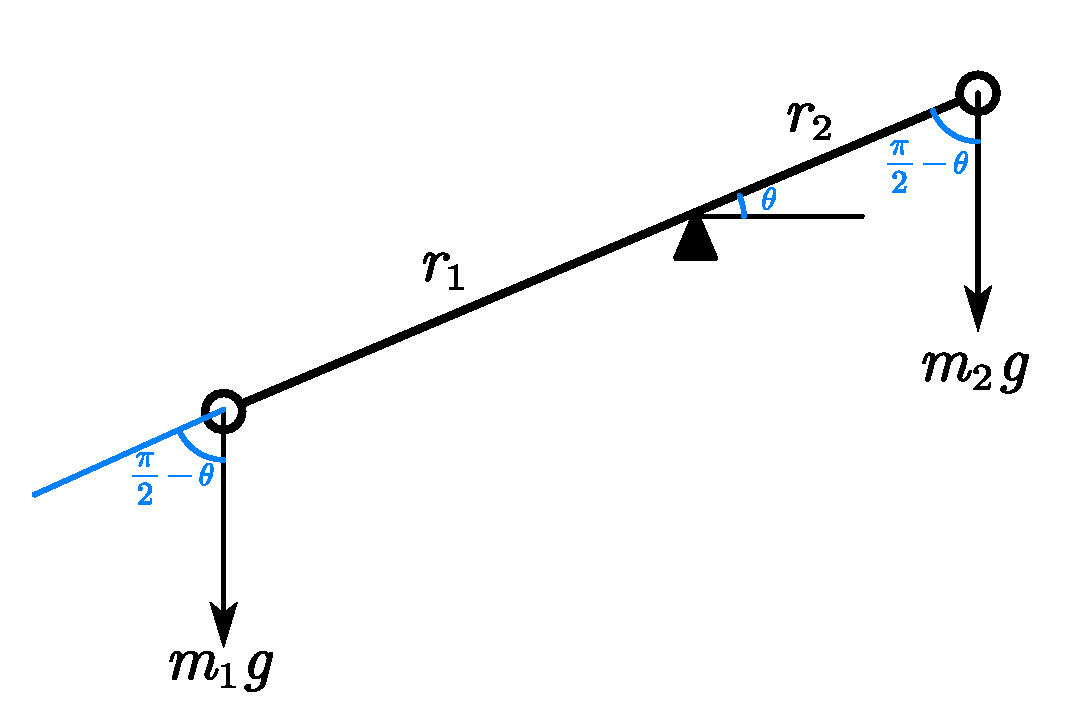
\includegraphics[width=6.5cm]{./figures/CM_1.pdf}
\caption{轻杆与两小球} \label{CM_fig1}
\end{figure}

解: 以逆时针为正, 合力矩为
\begin{equation}
M = r_1 m_1 g \cos\theta - r_2 m_2 g \cos\theta = (r_1 m_1 - r_2 m_2) g \cos\theta
\end{equation}
由\autoref{CM_eq6}, 括号中两项相等, 所以无论 $\theta$ 去何值, 合力矩都为 0.
\end{example}
我们把一般性的证明留到 “重心\upref{CenG}” 中.

\subsection{连续质量分布}
对连续质量分布,令密度关于位置的函数为 $\rho (\bvec r)$,总质量为密度的体积分 %(链接未完成)
\begin{equation}
M = \int \rho (\bvec r) \dd{V}
\end{equation}
要计算质心, 我们可以把整个物体划分为许多小块(微元), 如果每一块都很小, 我们可以假设第 $i$ 块的位置为 $\bvec r_i$, 密度为常数 $\rho(\bvec r_i)$, 体积为 $\Delta V_i$, 所以质量为 $\Delta m_i = \rho(\bvec r_i) \Delta V_i$. 我们把每个小块都用 $\bvec r_i$ 处的一个质量为 $\Delta m_i$ 的质点来代替, 那么质心为
\begin{equation}
\bvec r_c = \frac{1}{M} \sum_i \Delta m_i \bvec r_i = \frac{1}{M} \sum_i \bvec r_i \rho(\bvec r_i) \Delta V_i
\end{equation}
当所有的微元的体积都趋近于零时, 我们就可以将该式用体积分\upref{IntN}表示为
\begin{equation}\label{CM_eq9}
\bvec r_c = \frac{1}{M}\int \bvec r\rho (\bvec r) \dd{V}
\end{equation}

这个积分中的被积函数是矢量, 结果也是矢量, 该如何计算呢? 答案就是像\autoref{CM_eq11} 那样分别对矢量的每个分量积分, 得到结果的每个分量(可见求和具有的性质, 积分通常也有).
\begin{equation}
\leftgroup{
x_c &= \frac{1}{M}\iiint x \sigma (\bvec r) \dd{x}\dd{y}\dd{z}\\
y_c &= \frac{1}{M}\iiint y \sigma (\bvec r) \dd{x}\dd{y}\dd{z}\\
z_c &= \frac{1}{M}\iiint z \sigma (\bvec r) \dd{x}\dd{y}\dd{z}
}\end{equation}

如果要计算的物体是一个厚度可以忽略不计的薄片, 令 $\sigma(\bvec r)$ 为面密度(单位面积的质量), 我们就可以用面积分代替体积分.
\begin{equation}\label{CM_eq10}
\bvec r_c = \frac{1}{M}\int \bvec r\sigma (\bvec r) \dd{S}
\end{equation}
即
\begin{equation}
\leftgroup{
x_c &= \frac{1}{M}\iint x \sigma (\bvec r) \dd{x}\dd{y}\\
y_c &= \frac{1}{M}\iint y \sigma (\bvec r) \dd{x}\dd{y}
}\end{equation}

\begin{example}{长方形的质心}\label{CM_ex2}
在平面直角坐标系中, 长方形均匀薄片的 4 个点分别为 $(0, 0)$, $(a, 0)$, $(a, b)$, $(b, 0)$, 面密度 $\sigma$ 为常数, 试计算其质心.

解: 长方形的总质量为 $M = ab \sigma$. 使用\autoref{CM_eq10} (分别对矢量的两个分量积分)得
\begin{equation}
x_c = \frac{1}{ab \sigma} \int_0^b \int_0^a x \sigma \dd{x} \dd{y}
= \frac{1}{a} \int_0^a x \dd{x} = \frac{a}{2}
\end{equation}
\begin{equation}
y_c = \frac{1}{ab \sigma} \int_0^b \int_0^a y \sigma \dd{x} \dd{y}
= \frac{1}{b} \int_0^b y \dd{y} = \frac{b}{2}
\end{equation}
可见质心的坐标为 $(a/2, b/2)$, 恰好在长方形的中心.
\end{example}

我们再补充两个例子用于练习积分的运算
\begin{example}{三角形的质心}
在平面直角坐标系中, 三角形均匀薄片的 3 个点分别为 $(-a, 0)$, $(b, 0)$, $(0, c)$. 试计算其质心.

解: 令面密度 $\sigma$ 为常数, 则总质量为 $M = (a+b)c \sigma / 2$. 两条斜边的直线方程分别为
\begin{equation}
x = f_1(y) = a(y-c)/c
\qquad
x = f_2(y) = b(c-y)/c
\end{equation}
做面积分得(先积 $x$ 再积 $y$)
\begin{equation}
\ali{
x_c &= \frac{2}{(a+b)c \sigma} \int_0^c \int_{f_1(y)}^{f_2(y)} x \sigma \dd{x} \dd{y}\\
&= \frac{1}{(a+b)c} \int_0^c [f_2^2(y) - f_1^2(y)] \dd{y} = \frac{b - a}{3}
}\end{equation}
\begin{equation}
\ali{
y_c &= \frac{2}{(a+b)c \sigma} \int_0^c \int_{f_1(y)}^{f_2(y)} y \sigma \dd{x} \dd{y}\\
&= \frac{2}{(a+b)c} \int_0^c [f_2(y) - f_1(y)] y \dd{y} = \frac{c}{3}
}\end{equation}
不难发现, 这就是初中所学的三角形的重心, 即底边中线的三等分点, 或三条中线的交点.
\end{example}

% 未完成: 扇形的质心

由于质点系的积分和求和具有同样的性质, 在以下的证明中, 我们只需对质点系加以证明, 结论对于连续质量分布的物体也同样适用.

\subsection{质心的唯一性}
既然质心的定义取决于参考系(因为 $\bvec r_i$ 取决于参考系),那么不同参考系中计算出的质心是否是空间中的同一点呢? 例如将\autoref{CM_ex2} 中的长方形平移 $\Delta s$, 质心是否也会平移 $\Delta s$? 我们只需要证明,在 $A$ 坐标系中得到的质心 $\bvec r_{Ac}$ 与 $B$ 坐标系中得到的质心 $\bvec r_{Bc}$ 满足关系
\begin{equation}\label{CM_eq4}
\bvec r_{Ac} = \bvec r_{AB} + \bvec r_{Bc}
\end{equation}
其中 $\bvec r_{AB}$ 是 $A$ 系原点指向 $B$ 系原点的矢量. 首先根据定义
\begin{equation}
\bvec r_{Ac} = \frac{1}{M}\sum_i m_i \bvec r_{Ai}  \qquad \bvec r_{Bc} = \frac{1}{M}\sum_i  m_i \bvec r_{Bi} 
\end{equation}
由位矢的坐标系变换%(未完成: 确保有介绍)
,$\bvec r_{Ai} = \bvec r_{AB} + \bvec r_{Bi}$, 所以
\begin{equation}
\bvec r_{Ac} = \frac{1}{M}\sum_i m_i(\bvec r_{AB} + \bvec r_{Bi})  = \bvec r_{AB} + \frac{1}{M} \sum_i m_i \bvec r_{Bi}  = \bvec r_{AB} + \bvec r_{Bc}
\end{equation}

\subsection{质心参考系}
定义质点系的\textbf{质心参考系}(或\textbf{质心系})为原点固定在质心上且没有转动的参考系(平动参考系).%链接未完成: 平动是相对的, 转动是绝对的.
根据质心的唯一性(\autoref{CM_eq4}),在质心系中计算质心(\autoref{CM_eq1}) 仍然落在原点,即
\begin{equation}\label{CM_eq7}
\sum_i m_i \bvec r_{ci} = \bvec 0
\end{equation}
其中 $\bvec r_{ci}$ 是质心系中质点 $i$ 的位矢.

注意质心系并不一定是惯性系,只有当合外力为零质心做匀速直线运动时,质心系才是惯性系.在非惯性系中,每个质点受惯性力.

\subsection{质心系中总动量}
把\autoref{CM_eq7} 两边对时间求导,得
\begin{equation}\label{CM_eq8}
\sum_i m_i \bvec v_{ci} = \bvec 0
\end{equation}
注意到等式左边是质心系中质点系的总动量,所以我们得到质心系的一个重要特点,\textbf{质心系中总动量为零}.
